\subsection{Graph 4}\label{Graph4}

The final graph showcases how users are connected to ads. From marketing perspective, this could be the most important part. For example, we could see what advertisements are popular per country.

Insertion of the data is demonstrated with the function bellow.
\begin{listing}[H]
\caption{Advertisements graph -part 1}
\begin{minted}{Python}
def create_ad_graph(ad_dataframe):
    uri, user, password = get_creds(3)
    driver = GraphDatabase.driver(uri, auth=(user, password))

    create_user_query = "MERGE (:User {id: $userId})"
    create_country_query = "MERGE (:Country {name: $country})"
    create_team_query = 
        "MERGE (:Team {id: $teamId, name: $team, price: $price})"
    create_ad_query = "MERGE (:Ad {id: $adId, category: $adCategory})"
    create_user_country_relation_query = 
        "MATCH (u:User), (c:Country) WHERE 
            u.id = $userId AND 
            c.name = $country CREATE (u)-[:LIVES_IN]->(c)"
    create_user_team_relation_query = 
        "MATCH (u:User), (t:Team) WHERE 
            u.id = $userId AND 
            t.id = $teamId CREATE (u)-[:SUPPORTS]->(t)"
    create_team_ad_relation_query = 
        "MATCH (t:Team), (a:Ad) WHERE 
            t.id = $teamId AND 
            a.id = $adId CREATE (t)-[:SHOWS]->(a)"
\end{minted}
\end{listing}

\begin{listing}[H]
\caption{advertisements graph -part 2}
\begin{minted}{Python}
    queries = [
        (create_user_query, 
            ad_dataframe
            .select("userId")
            .distinct()),
        (create_country_query, 
            ad_dataframe
            .select("country")
            .distinct()),
        (create_team_query, 
            ad_dataframe
            .select("teamId", "team", "price")
            .distinct()),
        (create_ad_query, 
            ad_dataframe
            .select("adId", "adCategory")
            .distinct()),
        (create_user_country_relation_query, 
            ad_dataframe
            .select("userId", "country")),
        (create_user_team_relation_query, 
            ad_dataframe
            .select("userId", "teamId")),
        (create_team_ad_relation_query, 
            ad_dataframe
            .select("teamId", "adId"))
    ]

    with driver.session() as session:
        for query, data in queries:
            for row in data.collect():
                session.run(query, **row.asDict())
\end{minted}
\end{listing}

Filter that was applied in this case was top teams (based on users) and country they are in. With this information, query can be extended in order to see what advertisements are popular in top teams.
\begin{landscape}
    \begin{figure}[H]
        \includegraphics[scale=0.105]{img/Neo4j/graph3.png}
        \centering
        \caption{Graph 4}
        \label{fig:graph3}
    \end{figure}
\end{landscape}

\begin{listing}[H]
\caption{Cypher filter 4}
\begin{minted}{Cypher}
MATCH (n)
WHERE (n)-[:LIVES_IN|:SUPPORTS]->()
WITH n, SIZE((n)<-[:LIVES_IN|:SUPPORTS]-()) AS incomingCount
ORDER BY incomingCount DESC
LIMIT 10
MATCH (n)-[rel]->(m)
RETURN n, rel, m
\end{minted}
\end{listing}

\begin{landscape}
  \begin{figure}[H]
    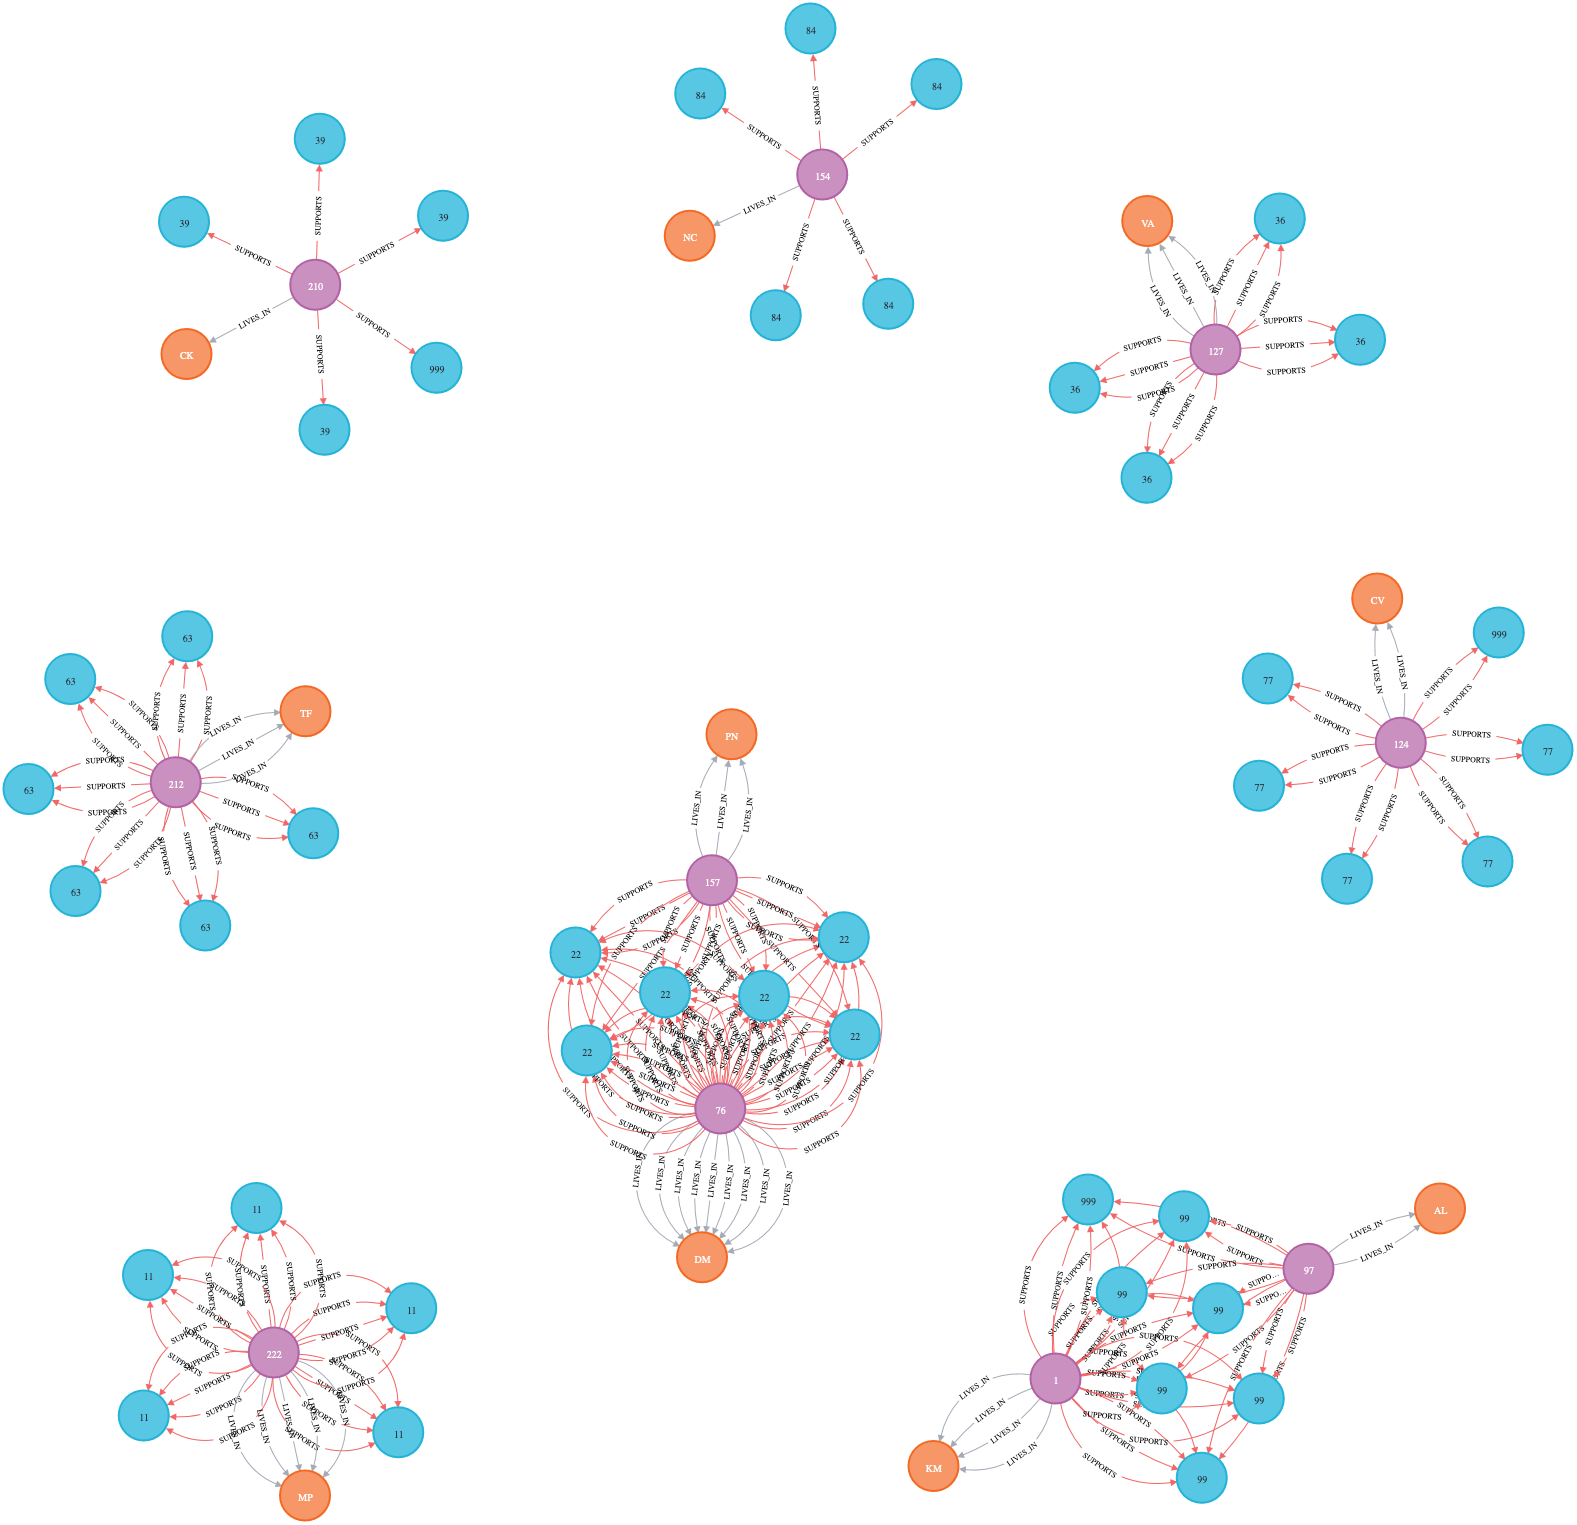
\includegraphics[scale=0.25]{img/Neo4j/graph3-filter.png}
    \centering
    \caption{Graph filtered 4}
    \label{fig:graph0}
  \end{figure}
\end{landscape}